%%
%\subsection{Perpendicular Bisectors}
\renewcommand{\theequation}{\theenumi}
\begin{enumerate}[label=\arabic*.,ref=\thesubsection.\theenumi]
\numberwithin{equation}{enumi}

\item Find a point $\vec{O}$ that is equidistant from the vertices of $\triangle ABC$ for $a = 5, b = 6, c = 4$.
%
\solution Let $\vec{O}$ be the desired point.  Then,
\begin{align}
\label{eq:tri_ccentre_def}
\norm{\vec{A}-\vec{O}} = \norm{\vec{B}-\vec{O}} = 
\norm{\vec{C}-\vec{O}} = R
%\\
%\implies \norm{\vec{x}-\vec{O}}^2 &=\brak{\vec{x}-\vec{O}}^T\brak{\vec{x}-\vec{O}} = R^2
\end{align}
From \eqref{eq:tri_ccentre_def},
\begin{align}
\label{eq:circle_const_AB}
\norm{\vec{A}-\vec{O}}^2 - \norm{\vec{B}-\vec{O}}^2  = 0
\end{align}
\begin{multline}
\implies \brak{\vec{A}-\vec{O}}^T\brak{\vec{A}-\vec{O}} 
\\
- \brak{\vec{B}-\vec{O}}^T\brak{\vec{B}-\vec{O}} = 0
\end{multline}
%
which can be simplified as
\begin{align}
\label{eq:circle_const_chord_ab}
\brak{\vec{A}-\vec{B}}^T\vec{O} =   \frac{\norm{\vec{A}}^2- \norm{\vec{B}}^2}{2}
\end{align}
Similarly,
\begin{align}
\label{eq:circle_const_chord_bc}
\brak{\vec{B}-\vec{C}}^T\vec{O} =   \frac{\norm{\vec{B}}^2- \norm{\vec{C}}^2}{2}
\end{align}
%
\eqref{eq:circle_const_chord_ab} and \eqref{eq:circle_const_chord_ab}, can be combined to form the matrix equation 
%
\begin{align}
\vec{N}^T\vec{O} &= \vec{c}
\\
\implies \vec{O} &= \vec{N}^{-T} \vec{c}
\label{eq:circle_const_chord_mat}
\end{align}
%
where 
%
\begin{align}
%\label{eq:circle_const_chord_mat}
\vec{N} &= \myvec{\vec{A}-\vec{B} & \vec{B}-\vec{C}}
\\
\vec{c} &= \frac{1}{2}\myvec{\norm{\vec{A}}^2- \norm{\vec{B}}^2 \\ \norm{\vec{B}}^2- \norm{\vec{C}}^2}
\end{align}
%
$\vec{O}$ can be computed using 
%
the python code below
%
\begin{lstlisting}
codes/circle/tri_ccentre.py
\end{lstlisting}
%
and the equivalent latex-tikz code to draw Fig. \ref{fig:tri_ccentre} is
%
\begin{lstlisting}
figs/triangle/tri_ccentre.tex
\end{lstlisting}
%
\begin{figure}[!ht]
	\begin{center}
		
		\resizebox{\columnwidth}{!}{%Code by GVV Sharma
%December 9, 2019
%released under GNU GPL
%Locating the circumcentre

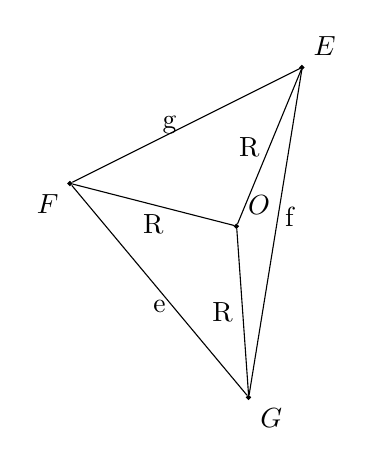
\begin{tikzpicture}
[scale=3.5,>=stealth,point/.style={draw,circle,fill = black,inner sep=0.5pt},]

%Triangle sides
\def\e{1.010}
\def\f{1.212}
\def\g{0.940}
 
%Coordinates of A
%\def\p{{\a^2+\c^2-\b^2}/{(2*\a)}}
%\def\p{0.5}
%\def\q{{sqrt(\c^2-\p^2)}}

%Labeling points
\node (E) at (5.313,2.657)[point,label=above right:$E$] {};
\node (F) at (4.471,2.236)[point,label=below left:$F$] {};
\node (G) at (5.119,1.460)[point,label=below right:$G$] {};

%Circumcentre

\node (O) at (5.075,2.081)[point,label=above right:$O$] {};

%Drawing triangle EFG
\draw (E) -- node[left] {$\textrm{g}$} (F) -- node[below] {$\textrm{e}$} (G) -- node[right,yshift=2mm] {$\textrm{f}$} (E);
%Drawing OA, OB, OC
\draw (O) -- node[left] {$\textrm{R}$} (E);
\draw (O) -- node[below] {$\textrm{R}$} (F);
\draw (O) -- node[left] {$\textrm{R}$} (G);

%\tkzMarkAngle[fill=blue!50,size=.3](C,B,O)
%\tkzMarkAngle[fill=blue!50,size=.3](O,C,B)


%\tkzMarkAngle[fill=red!50](O,A,C)
%\tkzMarkAngle[fill=red!50](A,C,O)


%\tkzMarkAngle[fill=orange!50,size=.3](B,A,O)
%\tkzMarkAngle[fill=orange!50,size=.3](O,B,A)

%\tkzLabelAngle[pos=0.5](O,C,B){$\theta_1$}
%\tkzLabelAngle[pos=0.5](O,B,C){$\theta_1$}
%\tkzLabelAngle[pos=0.5](O,A,B){$\theta_2$}
%\tkzLabelAngle[pos=0.5](O,B,A){$\theta_2$}
%\tkzLabelAngle[pos=1.5](O,A,C){$\theta_3$}
%\tkzLabelAngle[pos=1.5](O,C,A){$\theta_3$}

\end{tikzpicture}
}
	\end{center}
	\caption{Circumcentre $O$ of $\triangle ABC$}
	\label{fig:tri_ccentre}	
\end{figure}
%
\item In $\triangle OBC$, $OB = OC = R$.  Such a triangle is known as an {\em isoceles triangle}.
%
\item Show that $\angle OBC = \angle OCB$.  In an isoceles triangle, opposite sides and corresponding opposite angles are equal.
\label{prob:tri_ang_side_eq}
\\
\solution Using the sine formula in \eqref{eq:tri_sin_form},%
\begin{align}
\frac{\sin \angle OBC}{R} &= \frac{\sin \angle OCB}{R}
\\
\implies \sin \angle OBC &= \sin \angle OCB
\end{align}
%
\item  Show that $\angle BOC = 2\angle A$.
\label{prob:tri_ccentre_subtend}
%
\\
\solution In Fig. \ref{fig:tri_ccentre}, 
%
\begin{align}
%
\label{eq:tri_ccentre_A23}
A &= \theta_2+\theta_3
\\
B &= \theta_1+\theta_2
\\
C &= \theta_3+\theta_1
\\
\implies 2\brak{\theta_1+\theta_2+\theta_3} &= A+B+C =180\degree
\\
\implies \theta_1+\theta_2+\theta_3 &= 90\degree
\label{eq:tri_ccentre_sum_123}
\end{align}
%
From \eqref{eq:tri_ccentre_A23} and \eqref{eq:tri_ccentre_sum_123},
%
\begin{align}
%
\label{eq:tri_ccentre_A1}
A &= 90\degree - \theta_1
\end{align}
%
Also, in $\triangle OBC$, all angles add up to $180\degree$.  Hence, 
%
\begin{align}
\angle BOC + 2\theta_1 &= 180\degree
\\
\implies \angle BOC &= 180\degree - 2\theta_1 = 2 \brak{90\degree - \theta_1}
%\\
%&
= 2\angle A
\end{align}
%
upon substituting from \eqref{eq:tri_ccentre_A1}.
%
\item Let $\vec{D}$ be the mid point of $BC$.  Show that $OD \perp BC$.
\label{prob:tri_perp_bisect}
%
\\
\solution From \eqref{eq:circle_const_chord_bc}, 
%
\begin{align}
\brak{\vec{B}-\vec{C}}^T\vec{O} &=   \frac{\norm{\vec{B}}^2- \norm{\vec{C}}^2}{2}
\\
\implies \brak{\vec{B}-\vec{C}}^T\vec{O} &=   \frac{1}{2}\brak{\vec{B}- \vec{C}}^T\brak{\vec{B}+ \vec{C}}
\\
\implies \brak{\vec{B}-\vec{C}}^T&\brak{\vec{O} - \frac{\vec{B}+\vec{C}}{2}} = 0
\\
\text{or, } \brak{\vec{B}-\vec{C}}^T&\brak{\vec{O} - \vec{D}} = 0
\end{align}
%
$\because \vec{D} = \frac{\vec{B}+\vec{C}}{2}$ is the mid point of $BC$.  From \eqref{eq:tri_baudh_orth} we then conclude that $OD \perp BC$.
%
\item Perpendicular bisectors of a triangle meet at the circumcentre.
%
\item In the isosceles $\triangle OBC$, if $BD = DC$, $OD \perp BC$.
\label{them:isos_pb}
\end{enumerate}

